%%% Grasping Novel Objects

\subsubsection{Grasping Novel Objects with a Dexterous Hand}
\label{sec:GraspingNovelObjects}

In this section we show the extension of our approach to adaptation of a dexterous grasp type from year one, which is the other modus operandi we followed to tackle Task 4.3. We now solve two problems: {\em grasp type selection} and {\em adaptation of a grasp type}. The complete method enables learning of several grasp types, each from one kinesthetic demonstration. Thus the grasp type learning is one-shot. When presented with a novel object in any orientation the grasp generation algorithm generates hundreds of candidate grasps from each grasp type and ranks them according to likelihood. The extended method has been implemented on Boris, the bimanual robot platform at Birmingham (using a DLR-HIT Hand II) , having previously been tested on the Innsbruck robot with a different hand (Schunk 3-finger hand).

%% history, and why we're different --- Related work goes here
Previous work in learning generalisable grasps falls broadly into two classes. One class of approaches utilises the shape of common object parts or their appearance to generalise grasps across object categories \cite{saxena2008b,detry2013a,herzog2014a, kroemer2012a}. This works well for low DoF hands. Another class of approaches captures the global properties of the hand shape either at the point of grasping, or during the approach \cite{ben2012generalization}. This global hand shape can additionally be associated with global object shape, allowing generalisation by warping grasps to match warps of global object shape \cite{hillenbrand2012transferring}. This second class works well for high DoF hands, but generalisation is more limited. We achieve the advantages of both classes, generalising grasps across object categories with high DoF hands.

%% brief, condensed description of the contents which is in the paper
Both the learning and generation stages of our approach use an incomplete point cloud from a depth camera -- no prior model of object shape is used. As previously, the learned model is a product of experts, in which experts are of two types. The first is a {\em contact model} and is a density over the pose of a single hand link relative to the local object surface. The second is the {\em hand configuration model} and is a density over the whole hand configuration. 
%
The grasp inference implementation for novel objects (grasp transfer), which optimises the product of these two model types, has been improved to make it faster, generating thousands of grasp candidates in seconds. Also with improvements in computing power the time to compute a set of grasps has been reduced by a factor of more than 10. The key step in grasp transfer is the computation of a {\em query density} for each hand link. This is achieved by a Monte Carlo procedure that convolves the point cloud for the new object with the expert for an individual hand link. 
%An example of the resulting query density is given in Figure~\ref{fig:grasping.querydensity}. In this case the training grasp was on the rim of a wooden bowl, and the query object is a kettle.
%
%% this is Fig.7 of the paper: we could avoid it here
%\begin{figure}[!t]
%    \centerline{
%        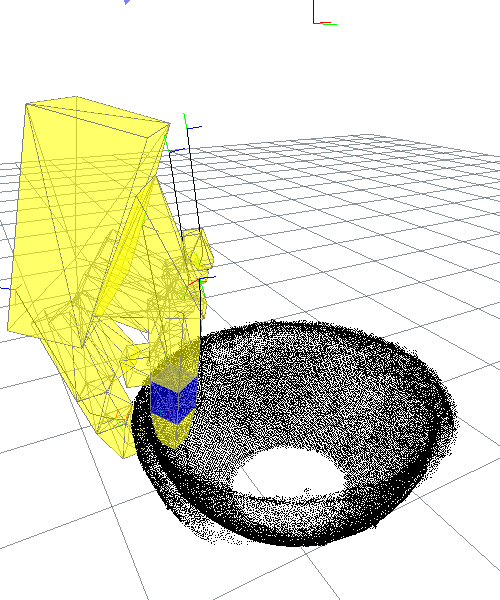
\includegraphics[height=3.5cm]{boris-v7/bowllarge/pinchsupp/link3}
%        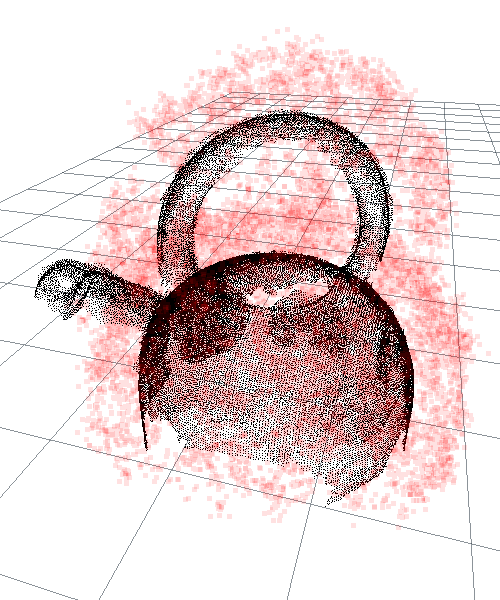
\includegraphics[height=3.5cm]{boris-v7/kettle/pinchsupp/link3-query}
%        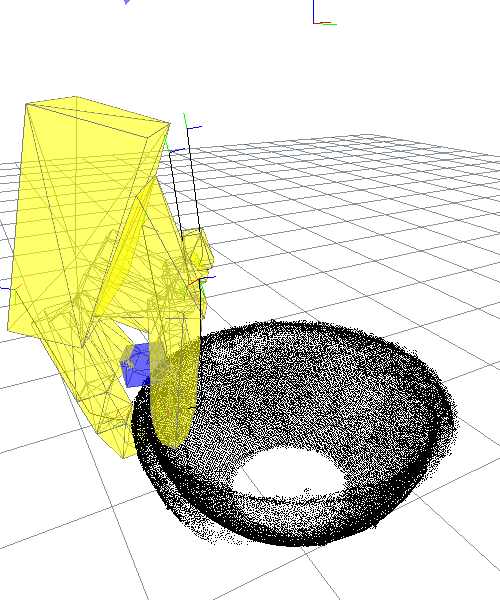
\includegraphics[height=3.5cm]{boris-v7/bowllarge/pinchsupp/link11}
%        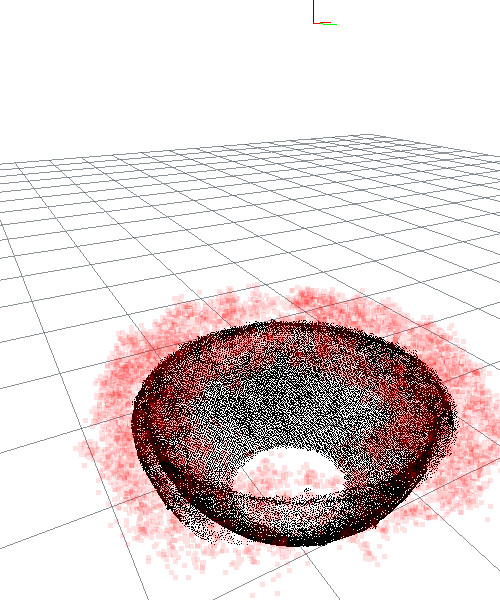
\includegraphics[height=3.5cm]{boris-v7/kettle/pinchsupp/link11-query}
%    }
%    \caption[Query density]{Visualisation of two query densities (panels 2 and 4 from the left) for two contact models (panels 1 and 3) of a pinch with support grasp. The links to which the contact models are associated are in blue. A query density is a distribution over poses of the corresponding link (red cloud) for a new ``query'' kettle.}
%    \label{fig:grasping.querydensity}
%\end{figure}

% experimental work
In experiments with Boris, the training set consisted of five different grasps, and the test set of forty-five previously unseen objects. The success rate of the first choice grasp is 77.7\% using a single view of the test object, and increases to 84.4\% if seven views are taken instead.
%Some example test grasps are given in Figure~\ref{fig:testing}.
%
%% this is Fig.9 of the paper: we could avoid it here
%\begin{figure}[p]
%    \newcommand{\testingw}{0.16\linewidth}
%    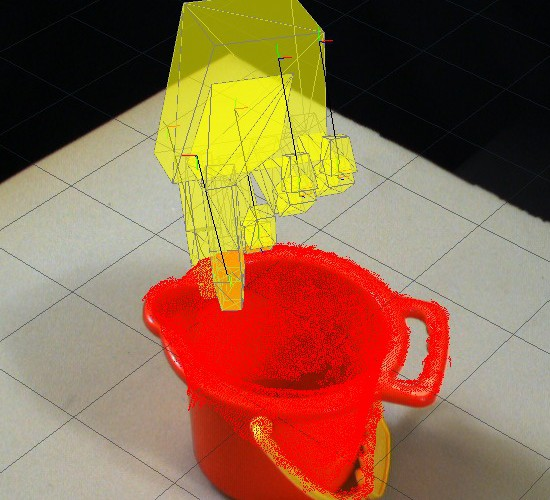
\includegraphics[width=\testingw]{boris-v7-crop/bucket/_cropped_screen000027} 
%    \includegraphics[width=\testingw]{boris-v7-crop/bucket/{_cropped_data-3201.851-externPointGrey.3}.jpg} 
%    \includegraphics[width=\testingw]{boris-v1-crop/bucket/_cropped_ri} 
%    \includegraphics[width=\testingw]{boris-v1-crop/bucket/{_cropped_datav1-1930.496-externpointgrey3}.jpg} 
%    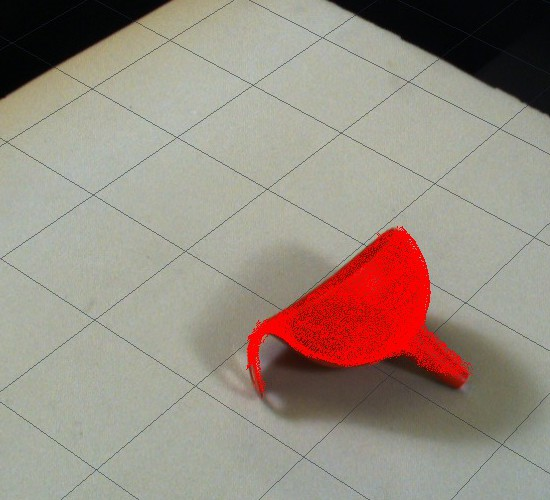
\includegraphics[width=\testingw]{boris-v7-crop/coke/_cropped_screen000051} 
%    \includegraphics[width=\testingw]{boris-v7-crop/coke/{_cropped_data-5546.733-externPointGrey.3}.jpg} 
%    \\
%    \includegraphics[width=\testingw]{boris-v1-crop/coke/_cropped_ri} 
%    \includegraphics[width=\testingw]{boris-v1-crop/coke/{_cropped_datav1-2959.660-externpointgrey3}.jpg} 
%    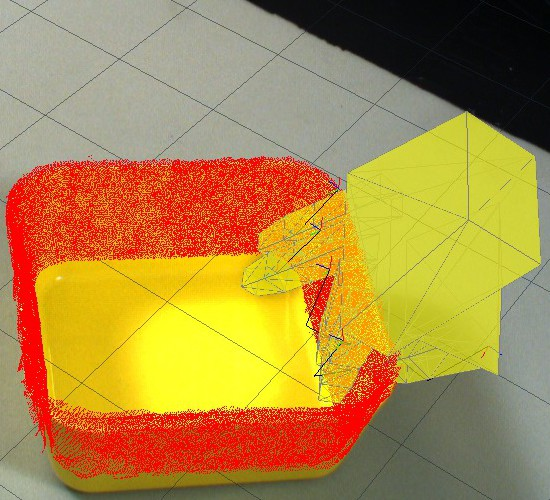
\includegraphics[width=\testingw]{boris-v7-crop/container1/_cropped_screen000016} 
%    \includegraphics[width=\testingw]{boris-v7-crop/container1/{_cropped_data-1839.940-externPointGrey.3}.jpg} 
%    \includegraphics[width=\testingw]{boris-v1-crop/container1/_cropped_ri} 
%    \includegraphics[width=\testingw]{boris-v1-crop/container1/{_cropped_datav1-4038.264-externpointgrey3}.jpg} 
%    \\
%    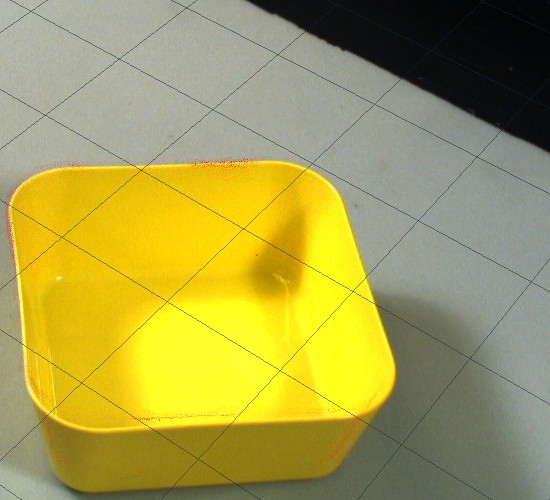
\includegraphics[width=\testingw]{boris-v7-crop/cup2/_cropped_screen000013} 
%    \includegraphics[width=\testingw]{boris-v7-crop/cup2/{_cropped_data-438.213-externPointGrey.3}.jpg} 
%    \includegraphics[width=\testingw]{boris-v1-crop/cup2/_cropped_ri} 
%    \includegraphics[width=\testingw]{boris-v1-crop/cup2/{_cropped_datav1-5208.103-externpointgrey3}.jpg} 
%    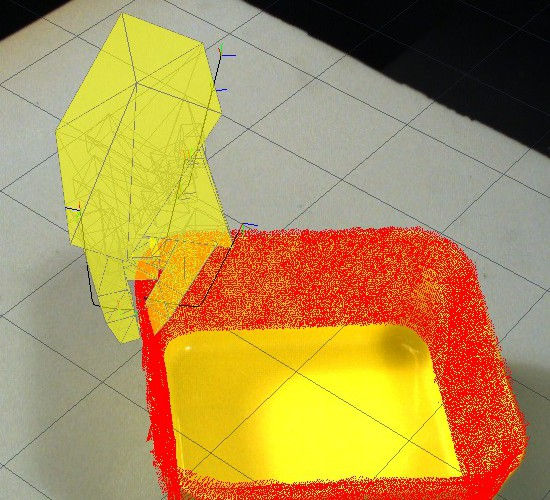
\includegraphics[width=\testingw]{boris-v7-crop/guttering/_cropped_screen000014} 
%    \includegraphics[width=\testingw]{boris-v7-crop/guttering/{_cropped_data2-148.522-externPointGrey.3}.jpg} 
%    \\
%    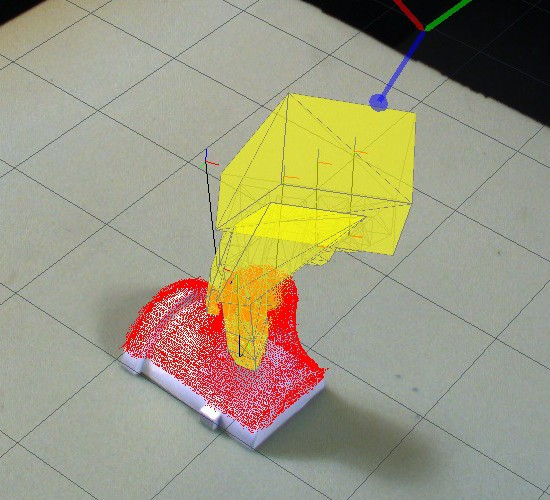
\includegraphics[width=\testingw]{boris-v7-crop/guttering/_cropped_screen000004}
%    \includegraphics[width=\testingw]{boris-v7-crop/guttering/{_cropped_data-585.300-externPointGrey.3}.jpg}
%    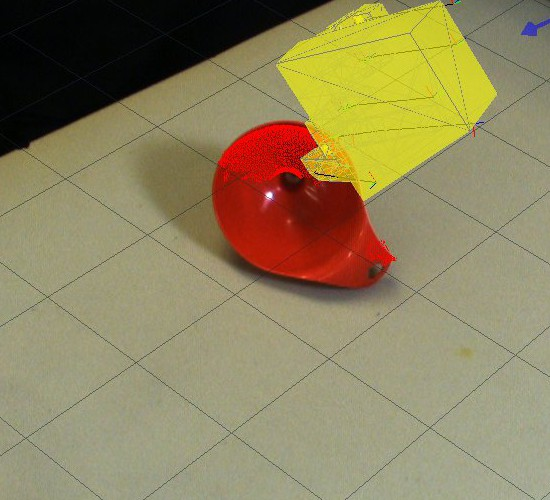
\includegraphics[width=\testingw]{boris-v1-crop/guttering/_cropped_side-gri} 
%    \includegraphics[width=\testingw]{boris-v1-crop/guttering/{_cropped_datav12-5768.286-externpointgrey3}.jpg} 
%    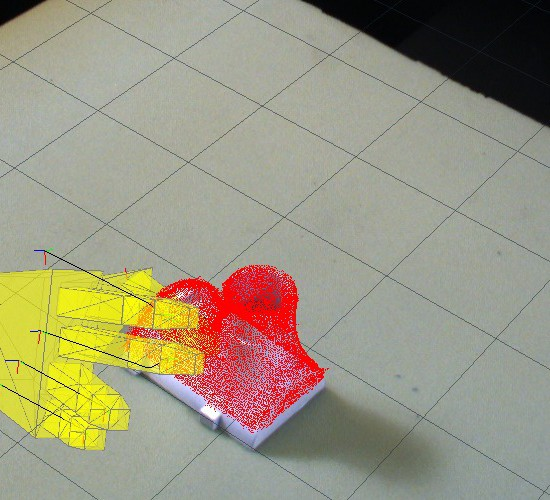
\includegraphics[width=\testingw]{boris-v7-crop/mrmuscle/_cropped_screen000007} 
%    \includegraphics[width=\testingw]{boris-v7-crop/mrmuscle/{_cropped_data-353.435-externPointGrey.3}.jpg} 
%    \\
%    \includegraphics[width=\testingw]{boris-v1-crop/mrmuscle/_cropped_ri} 
%    \includegraphics[width=\testingw]{boris-v1-crop/mrmuscle/{_cropped_datav1-4510.631-externpointgrey3}.jpg} 
%    %\\
%    %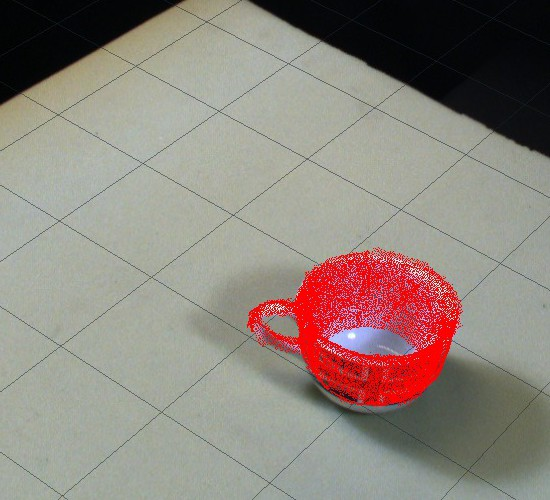
\includegraphics[width=\testingw]{boris-v7-crop/mug1/_cropped_screen000010}
%    %\includegraphics[width=\testingw]{boris-v7-crop/mug1/{_cropped_data2-1739.597-externPointGrey.3}.jpg}
%    %\includegraphics[width=\testingw]{boris-v1-crop/mug1/_cropped_ri}
%    %\includegraphics[width=\testingw]{boris-v1-crop/mug1/{_cropped_datav1-101.071-externpointgrey3}.jpg}
%    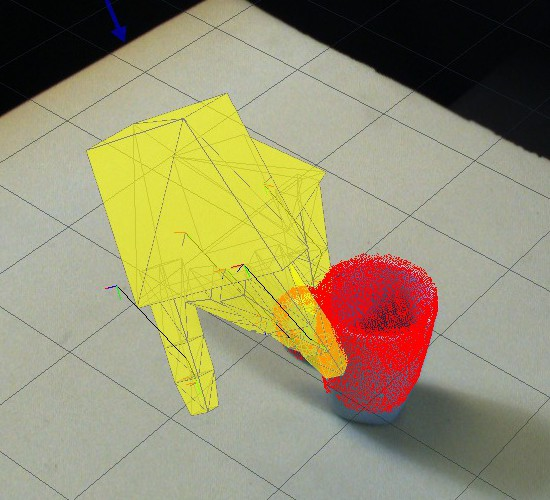
\includegraphics[width=\testingw]{boris-v7-crop/mug4/_cropped_screen000003} 
%    \includegraphics[width=\testingw]{boris-v7-crop/mug4/{_cropped_data-154.877-externPointGrey.3}.jpg} 
%    \includegraphics[width=\testingw]{boris-v1-crop/mug4/_cropped_ri} 
%    \includegraphics[width=\testingw]{boris-v1-crop/mug4/{_cropped_datav1-1758.848-externpointgrey3}.jpg} 
%    \\
%    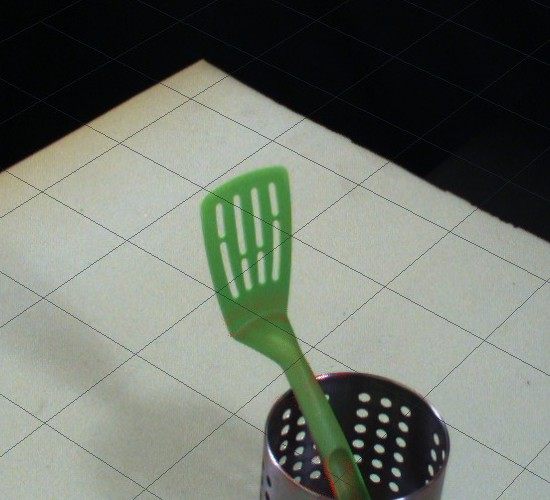
\includegraphics[width=\testingw]{boris-v7-crop/saucepanlarge/_cropped_screen000065}  
%    \includegraphics[width=\testingw]{boris-v7-crop/saucepanlarge/{_cropped_data-3841.539-externPointGrey.3}.jpg}  
%    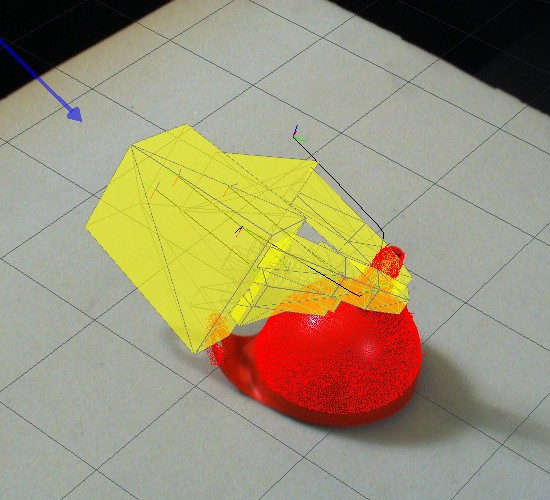
\includegraphics[width=\testingw]{boris-v7-crop/funnellarge/_cropped_screen000038} 
%    \includegraphics[width=\testingw]{boris-v7-crop/funnellarge/{_cropped_data-1856.011-externPointGrey.3}.jpg} 
%    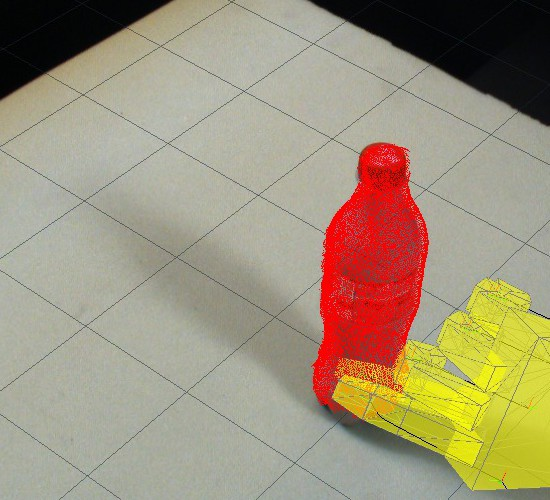
\includegraphics[width=\testingw]{boris-v7-crop/funnellarge/_cropped_screen000054} 
%    \includegraphics[width=\testingw]{boris-v7-crop/funnellarge/{_cropped_data2-3498.448-externPointGrey.3}.jpg} 
%    \\
%    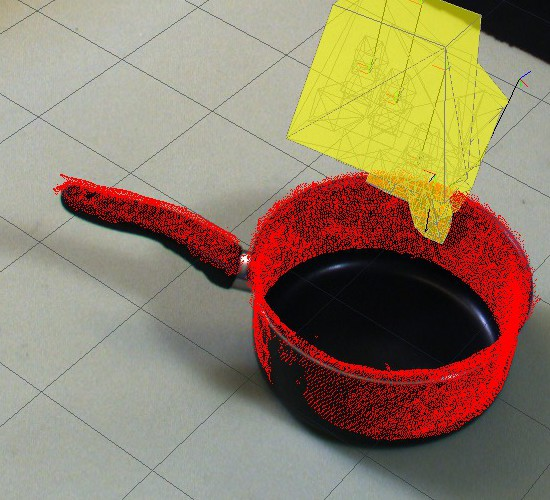
\includegraphics[width=\testingw]{boris-v7-crop/spatula/_cropped_screen000071} 
%    \includegraphics[width=\testingw]{boris-v7-crop/spatula/{_cropped_data3-4065.617-externPointGrey.3}.jpg} 
%    \includegraphics[width=\testingw]{boris-v1-crop/spatula/_cropped_ri} 
%    \includegraphics[width=\testingw]{boris-v1-crop/spatula/{_cropped_datav1-444.576-externpointgrey3}.jpg} 
%    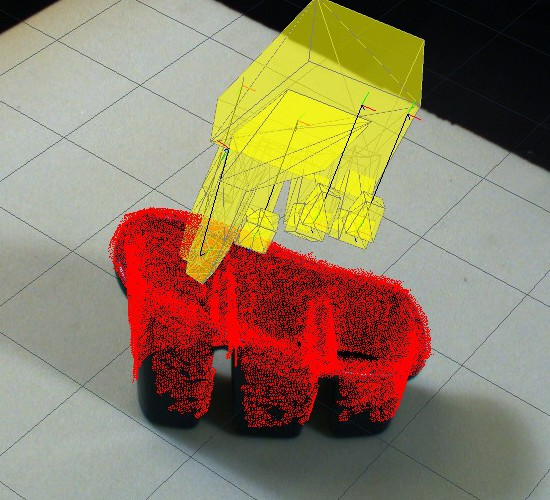
\includegraphics[width=\testingw]{boris-v7-crop/stand1/_cropped_screen000075}  
%    \includegraphics[width=\testingw]{boris-v7-crop/stand1/{_cropped_data-4588.209-externPointGrey.3}.jpg}  
%    \\
%    \includegraphics[width=\testingw]{boris-v1-crop/stand1/_cropped_ri}   
%    \includegraphics[width=\testingw]{boris-v1-crop/stand1/{_cropped_datav1-791.865-externpointgrey3}.jpg}   
%    %\includegraphics[width=\testingw]{boris-v7-crop/tongs/_cropped_screen000054}
%    %\includegraphics[width=\testingw]{boris-v7-crop/tongs/{_cropped_data3-2655.581-externPointGrey.3}.jpg}
%    %\includegraphics[width=\testingw]{boris-v1-crop/tongs/_cropped_ri}
%    %\includegraphics[width=\testingw]{boris-v1-crop/tongs/{_cropped_datav1-874.232-externpointgrey3}.jpg}
%    %\\
%    \includegraphics[width=\testingw]{boris-v7-crop/wineglass/_cropped_screen000042}  
%    \includegraphics[width=\testingw]{boris-v7-crop/wineglass/{_cropped_data-2118.818-externPointGrey.3}.jpg}  
%    \includegraphics[width=\testingw]{boris-v1-crop/wineglass/_cropped_ri}  
%    \includegraphics[width=\testingw]{boris-v1-crop/wineglass/{_cropped_datav1-2051.782-externpointgrey3}.jpg}  
%    \caption{The test objects with a visualisation of some of the successful grasps. Each grasp is shown by a pair of images, with the visualisation of the planned grasp and the obtained point cloud on the left, and the actual grasp execution on the right. Those from the 7 view and 1 view conditions can easily be distinguished by the proportion of the object covered by the recovered point cloud.}
%    \label{fig:testing}
%\end{figure}

More details on the highlighted method and the experimental results can be found in the attached paper~\cite{kopicki2015oneshot} available at this~\href{./attachedPapers/GraspingNovelObjects.pdf}{link}. 
